\documentclass{article}
\usepackage[a4paper, margin=1mm, landscape]{geometry}
\usepackage{multicol}
\usepackage{xcolor}
\usepackage{enumitem}
\usepackage{amsmath}
\usepackage{amsfonts}
\usepackage{listings}
\usepackage{soul}
\usepackage{graphicx}

\pdfinfo{
    /Title (CS4243.pdf)
    /Creator (TeX)
    /Producer (pdfTeX 1.40.0)
    /Author (Jason Qiu)
    /Subject (CS4243)
    /Keywords (CS4243, nus, cheatsheet, pdf)
}

\graphicspath{ {./img/} }

\pagestyle{empty}
\setcounter{secnumdepth}{0}
\setlength{\columnseprule}{0.25pt}

% Redefine section commands to use less space
\makeatletter
\renewcommand{\section}{\@startsection{section}{1}{0mm}%
    {-1ex plus -.5ex minus -.2ex}%
    {0.5ex plus .2ex}%x
{\normalfont\large\bfseries}}
\renewcommand{\subsection}{\@startsection{subsection}{2}{0mm}%
    {-1explus -.5ex minus -.2ex}%
    {0.5ex plus .2ex}%
{\normalfont\normalsize\bfseries}}
\renewcommand{\subsubsection}{\@startsection{subsubsection}{3}{0mm}%
    {-1ex plus -.5ex minus -.2ex}%
    {1ex plus .2ex}%
{\normalfont\small\bfseries}}%
\makeatother

% Adjust spacing for all itemize/enumerate
\setlength{\leftmargini}{0.5cm}
\setlength{\leftmarginii}{0.5cm}
\setlist[itemize,1]{leftmargin=2mm,labelindent=1mm,labelsep=1mm}
\setlist[itemize,2]{leftmargin=2mm,labelindent=1mm,labelsep=1mm,label=$\bullet$}
\setlist[itemize,3]{leftmargin=2mm,labelindent=1mm,labelsep=1mm,label=$\bullet$}
\setlist[enumerate,1]{leftmargin=2mm,labelindent=1mm,labelsep=1mm}
\setlist[enumerate,2]{leftmargin=2mm,labelindent=1mm,labelsep=1mm,label=(\arabic*)}
\setlist[itemize]{nolistsep}
\setlist[enumerate]{nolistsep}

% Adjust column separator width in matrix
\setlength{\arraycolsep}{2.5pt}

% Font
\renewcommand{\familydefault}{\sfdefault}

% Define colors for math formulas
\definecolor{myblue}{cmyk}{1,.72,0,.38}
\everymath\expandafter{\the\everymath \color{myblue}}

% Custom command for keywords
\definecolor{highlight}{RGB}{251,243,218}
\newcommand{\keyword}[2]{\sethlcolor{highlight}\hl{\textbf{#1}} - #2}
\newcommand{\ilkeyword}[1]{\sethlcolor{highlight}\hl{\textbf{#1}}}

% Define colors and style for code
\definecolor{codegreen}{rgb}{0,0.6,0}
\definecolor{codegray}{rgb}{0.5,0.5,0.5}
\definecolor{codered}{HTML}{CC241D}
\definecolor{backcolor}{rgb}{0.95,0.95,0.95}
\lstdefinestyle{codestyle}{
    backgroundcolor = \color{backcolor},
    commentstyle = \color{codegray},
    keywordstyle = \color{codered},
    stringstyle = \color{codegreen},
    basicstyle = \ttfamily,
    breakatwhitespace = false,
    showstringspaces = false,
    breaklines = true,
    showtabs = false,
    tabsize = 2
}
\lstset{style = codestyle}

% -----------------------------------------------------------------------
\begin{document}
\begin{multicols*}{4}
\footnotesize

% Title box
\begin{center}
    \fbox{
        \parbox{0.8\linewidth}{
            \centering \textcolor{black}{
                {\Large\textbf{CS4243}} \\
                \normalsize{AY23/24 Sem 2}} \\
                {\footnotesize \textcolor{gray}{github.com/jasonqiu212}}
        }
    }
\end{center}

\section{05. Segmentation}

\begin{itemize}
    \item Goal: Separate image into coherent regions
    \item Idea: \keyword{Clustering}{Group similar data points together}
    \item Challenges: What makes 2 points same/different? Choice of features (e.g. Color, Intensity, Position), Which clustering algorithm?
    \item \keyword{k-Means Clustering}{Iteratively re-assign points to nearest cluster center}
    \begin{enumerate}
        \item Randomly initialize the cluster centers $c_1, \ldots, c_K$
        \item For each point $p_i$, find the closest $c_j$ to put $p_i$ in
        \item Set $c_j$ to be mean of points in cluster $j$
        \item Repeat, if $c_j$ have changed up to some threshold
    \end{enumerate}
    \begin{itemize}
        \item Pros: Simple, Converges to local min.
        \item Cons: Setting $K$, Sensitive to initial centers (Since k-means converges to local min.), Sensitive to outliers (Can add more clusters), Assumes spherical clusters
    \end{itemize}
    \item \ilkeyword{Simple Linear Iterative Clustering (SLIC) Superpixels}
    \begin{itemize}
        \item \keyword{Superpixel}{Group of pixels that share common traits}
        \begin{itemize}
            \item Application: Inputs to other CV algo. since more compact representation with perceptual meaning
        \end{itemize}
        \item Num. of pixels: $n_{tp}$; Target num. of superpixels: $n_{sp}$
        \item Initial width of each superpixel: $s = \sqrt{n_{tp} / n_{sp}}$
        \item Features: $z = [r,g,b,x,y]$
        \item Color distance: $d_c = || \langle r_j,g_j,b_j \rangle - \langle r_i,g_i,b_i \rangle ||$
        \item Spatial distance: $d_s = || \langle x_j,y_j \rangle - \langle x_i,y_i \rangle ||$
        \item Scaling factors: $d_{cm}$ and $d_{sm}=s$ set as max. expected values of $d_c$ and $d_s$ respectively
        \item $D = \sqrt{(\frac{d_c}{d_{cm}})^2+(\frac{d_s}{d_{sm}})^2} = \sqrt{d_c^2 + (\frac{d_s}{s})^2 c^2}$
    \end{itemize}
    \begin{enumerate}
        \item Split img. into grid of size $s \times s$. Set cluster centers as lowest gradient position in $3 \times 3$ neighborhood from superpixel center to speed up convergence since initialize on value common to surrounding.
        \item For each cluster center, check distance to all pixels within $2s \times 2s$ neighborhood. Assign pixels to closest checked center.
        \item Update cluster centers using mean and repeat if not converged (Same as k-Means)
        \item Optional: Replace superpixel region by average value to create stained glass effect
    \end{enumerate}
    \begin{itemize}
        \item Modification of k-Means: Not random initialization, Compute pixel's distance only to closest set of cluster centers
        \item Can enforce connectivity and use other features too
    \end{itemize}
    \item \keyword{Mean-Shift Clustering}{Find local density maxima in feature space}
    \begin{itemize}
        \item \keyword{Attraction basin}{Region in feature space for which all trajectories of centroids lead to same mode}
        \item \keyword{Cluster}{All data points in attraction basin of a mode}
    \end{itemize}
    \begin{enumerate}
        \item For each data point:
        \begin{enumerate}
            \item Define window around and get centroid
            \item Shift window to centroid
            \item Repeat until window centroid stops moving
        \end{enumerate}
    \end{enumerate}
    \begin{itemize}
        \item Segmentation with Mean Shift: Do mean shift and merge pixels in same attraction basin
        \item Choosing window size: Trial and error, Sample points and use avg. dist. to knn. (Num. of neighbors needs to be large enough to ensure increase in density)
        \begin{itemize}
            \item Larger window size $\rightarrow$ Fewer clusters
        \end{itemize}
        \item Pros: No assumptions on cluster shape, 1 parameter, Finds variable num. of modes (vs. specified $k$ in k-Means), Robust to outliers
        \item Cons: Choosing $h$, Slow, Scales poorly with feature space dimension
        \item Optimizations:
        \begin{itemize}
            \item After each run of mean shift, assign all points within radius $r$ of end point to same cluster
            \item Assign points in radius $c < r$ of search path to mode
        \end{itemize}
    \end{itemize}
\end{itemize}

\section{06. Texture}

\begin{itemize}
    \item \keyword{Texture}{Pattern with repeating elements}
    \item \keyword{Filter Bank}{Measures variety of structures in local neighborhood and generates multi-dimensional features}
    \begin{itemize}
        \item Goal: How to represent texture?
        \item Idea: Apply filters with small windows to generate statistics that summarize local patterns. Dist. in feature space bet. windows $\rightarrow$ Pixel's texture similarity
        \item $d$ filters $\rightarrow$ $d$-dimensional feature vector
        \item Choosing window size: Try many sizes and look for one where statistic does not change much
        \item Choose filters in different scales and orientations (to solve window size problem)
        \item \keyword{Gabor Filter}{Represent filter banks mathematically by combining sinusoids with exp. (Gaussian) envelope}
    \end{itemize}
    \item \keyword{Texton}{Characterizes texture by replacing each pixel with integer representing \textbf{texture type}}
    \begin{enumerate}
        \item Apply filter bank to training image
        \item Cluster in feature space and store cluster centers (Texton dictionary)
        \item For test image, filter image with same filter bank to get feature vector for each pixel. Assign each pixel to nearest cluster. Cluster ID = Texton ID.
        \item For a given region, compute \ilkeyword{texton histograms}
    \end{enumerate}
    \begin{itemize}
        \item Classification: Given new img., compare hist. to other trng. samples and assign to label with most similarity
        \item Segmentation: Use texton histograms as a feature
    \end{itemize}
    \item \keyword{Perceived Boundaries}{Segmentation by human}
    \begin{itemize}
        \item Idea: Texture gradients indicate boundaries well
    \end{itemize}
    \begin{enumerate}
        \item For each pixel, consider a disk that is split into 2 halves with some orientation
        \item Measure texture diff. bet. 2 halves via texton hist.
        \item Try all orientations. Orientation with high difference suggests boundaries.
    \end{enumerate}
\end{itemize}

\section{07. Keypoints}

\begin{itemize}
    \item Motivation: How to stitch 2 images (e.g. Panaroma)?
    \begin{enumerate}
        \item Keypoints: Find locations
        \item Descriptors: Rep. surrounding regions with math
        \item Do the matching
    \end{enumerate}
    \item Good keypoints are \textbf{repeatable} and \textbf{distinct}
    \item \ilkeyword{Harris Corner Detection}
    \begin{itemize}
        \item Significance: Corners have big changes in all directions when shifting window
        \item Given window $W$ shifted by offset $(u,v)$:
        \[
            E(U,v)=\sum_{(x,y) \in W} (I(x+u,y+v) - I(x,y))^2
        \]
        \item Assuming only small shifts (for Taylor Series Exp.):
        \[
            E(u,v) = Au^2 + 2Buv + Cv^2 = \begin{bmatrix}
                u & v \\
            \end{bmatrix}
            \begin{bmatrix}
                A & B \\
                B & C \\
            \end{bmatrix}
            \begin{bmatrix}
                u \\
                v \\
            \end{bmatrix}
        \]
        \begin{itemize}
            \item $A = \sum_{(x,y) \in W} I_x^2$ $\quad$ $B = \sum_{(x,y) \in W} I_x I_y$
            \item $C = \sum_{(x,y) \in W} I_y^2$
            \item \keyword{2nd Moment Matrix (H)}{Middle matrix}
        \end{itemize}
        \item $E = k$ visualized as ellipse, where $H$ controls shape
            \begin{itemize}
                \item Eigenvectors of $H$ $\rightarrow$ Axes orientation
                \item Eigenvalues of $H$ $\rightarrow$ Axes length
            \end{itemize}
        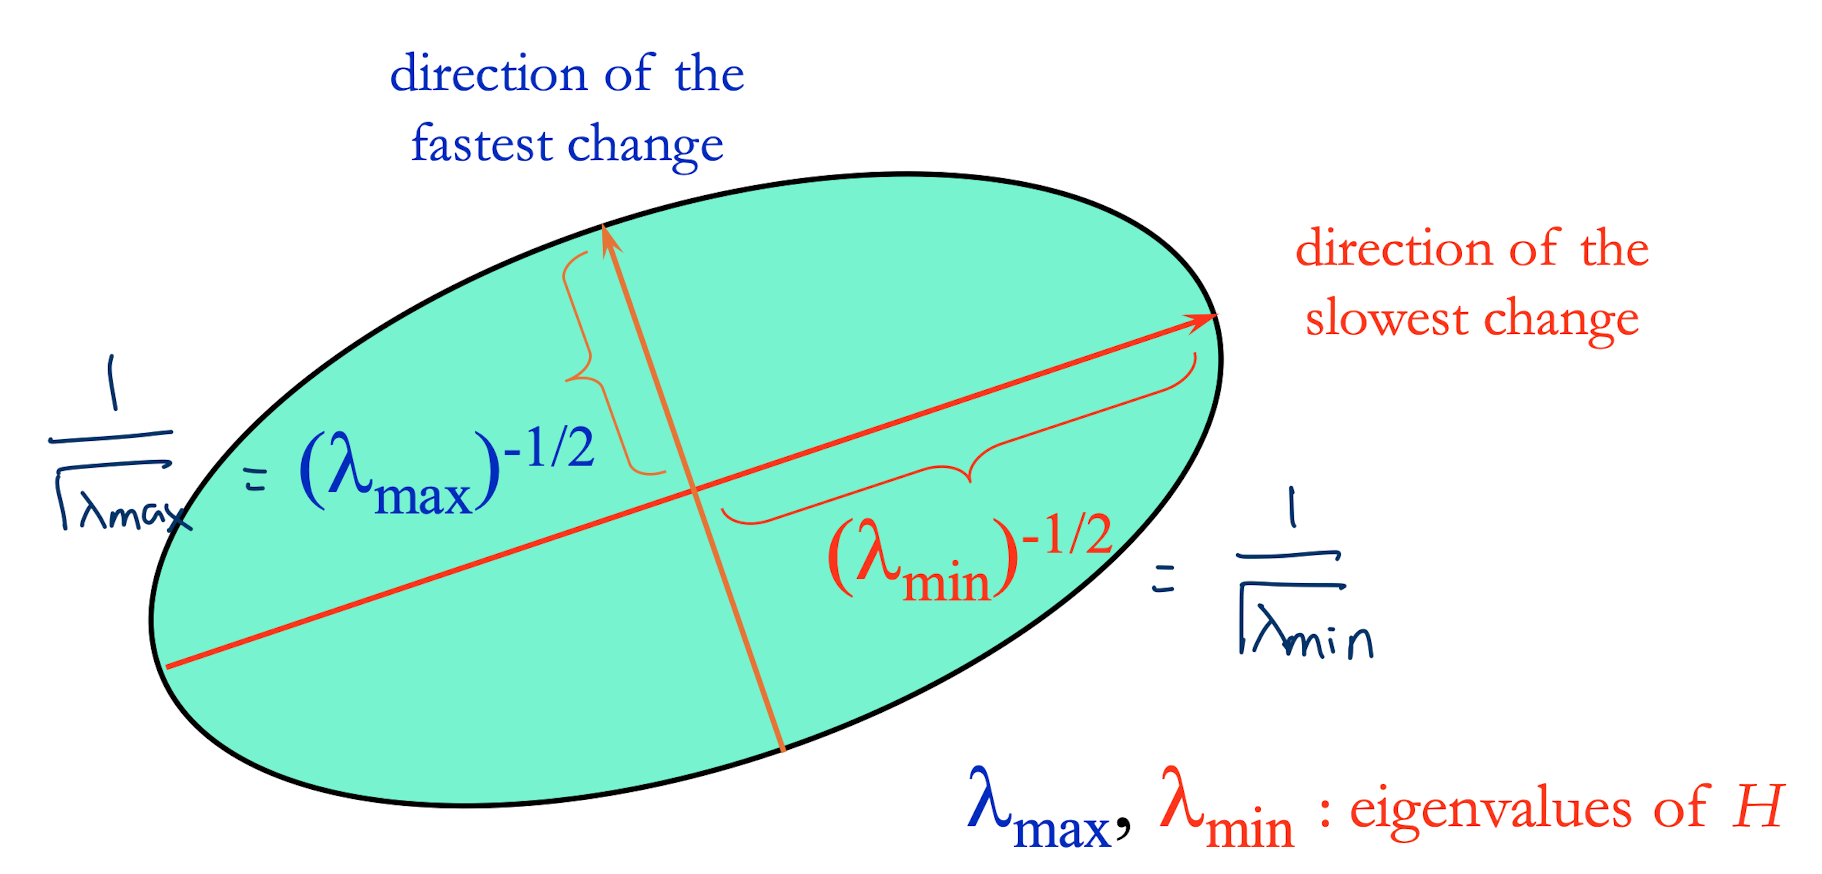
\includegraphics[scale=0.18]{h-ellipse.jpg}
        \item \ilkeyword{Eigenvectors} of $A$ are vectors $\mathbf{x}$ that: $A\mathbf{x} = \lambda \mathbf{x}$
        \item \ilkeyword{Eigenvalue ($\lambda$)} corresponds to $\mathbf{x}$: $\det(A-\lambda I) = 0$
        \item Since $A = H$ is $2 \times 2$: $\lambda_{\pm} = \frac{1}{2} ((h_{11} + h_{22}) \pm \sqrt{2h_{12}h_{21} + (h_{11} - h_{22})^2})$
        \item After getting $\lambda$s, find $\mathbf{x}$: $(A - \lambda I) \mathbf{x} = 0$
        \item Both $\lambda_{\text{max}}$ and $\lambda_{\text{min}}$ are large $\rightarrow$ Corner
        \item 'Cornerness' Score: $R = \min(\lambda_1, \lambda_2)$ (But getting $\lambda$ is slow)
        \item \ilkeyword{Harris Operator}: $R = \det (H) - \kappa (\text{trace}(H))^2$
        \begin{itemize}
            \item $\det (H) = AC - B^2 = \lambda_1 \lambda_2 $
            \item $\text{trace} (H) = A + C = \lambda_1 + \lambda_2 $
            \item $R > 0$ $\rightarrow$ Corner, $R<0$ $\rightarrow$ Edge, $R \approx 0$ $\rightarrow$ Flat
        \end{itemize}
        \begin{enumerate}
            \item Compute gradient for each point in image
            \item Compute $H$ matrix for each image window and get 'correctness' score
            \item Find points with window where $R > $ threshold
            \item Take points of local maxima
        \end{enumerate}
        \item \keyword{Non-Max. Suppression}{Iteratively search for max. values, then zero everything in surrounding window}
        \begin{itemize}
            \item Window size important
            \item Adaptive: To prevent uneven distri. of keypoints in areas of higher contrast, pick corners which are both local max. and whose response is greater than all neighboring local max.
        \end{itemize}
        \item In practice: $H = \sum_{(x,y) \in W} w_{x,y} \begin{bmatrix}
            I_x^2 & I_x I_y \\
            I_x I_y & I_y^2 \\
            \end{bmatrix}$ (e.g. Convolve with Gaussian)
    \end{itemize}
    \item \ilkeyword{Harris Corner Invariances}
    \begin{itemize}
        \item Purpose: If img. transf., how repeatable is detection?
        \item \keyword{Equivariance}{Image transformed, and detection location undergoes similar transformation}
        \item \keyword{Invariance}{Image tranf., but no detection score change}
        \item Translation: Equivariant and invariant
        \item Rotation: Equivariant and invariant
        \item Photometric transformation (Assume $I' = aI + b$): Invariant to $b \neq 0$, but not invariant to $a \neq 1$
        \item Scaling: Not equivariant and invariant
        \begin{itemize}
            \item Scale of window can determine if location is keypoint $\rightarrow$ Need to scale up window by image scale
            \item \keyword{Auto. Scale Selection}{When looking for keypoints, try window sizes and find scale that gives local max.}
        \end{itemize}
    \end{itemize}
    \item \keyword{Laplacian of Gaussian}{Alternative keypoint detector which detects 'blobs' and is scale-sensitive}
    \begin{itemize}
        \item $\nabla^2 g = \frac{\partial^2 g}{\partial x^2} + \frac{\partial^2 g}{\partial y^2}$
        \item Practice: Approx. by Difference of Gaussian for speed
        \item Idea: Convolution with LoG has highest response when signal has same scale as Gaussian. Built-in scale sensitivity by varying scale $\sigma$.
        \item Implementation: Fix window and kernel size; rescale img. with Gaussian blurring and downsampling
    \end{itemize}
\end{itemize}

\section{08. Descriptors}

\begin{itemize}
    \item Goal: Get feature vector surrounding each keypoint and measure similarity between feature vectors for matching
    \item Desc. should be invariant/equivariant and unique. E.g.:
    \begin{itemize}
        \item Raw intensity: Good for exact template matching, but sensitive to lighting
        \item Image gradient: Invariant to raw intensity (i.e. Lighting), but sensitive to transformations
        \item Color histogram: Invariant to scale and rotation, but not sensitive to spatial layout
        \item Spatial histogram: Compute color histograms over spatial cells. But not invariant to large rotations.
        \begin{itemize}
            \item Orientation normalization: Normalize orientation of patch based on dominant image gradient
            \item Save orien. angle $\theta$ w/ keypoint (e.g. Mean, mode)
        \end{itemize}
        \item \keyword{GIST Descriptor}{Rough spatial distribution of image gradients that is rotation invariant}
        \begin{enumerate}
            \item Divide image into $4 \times 4$ grid
            \item Apply Gabor filters (All dir. edge; $N$ filters)
            \item Compute filter response averages for each cells
            \item Size of descriptor: $4 \times 4 \times N$
        \end{enumerate}
    \end{itemize}
    \item \keyword{SIFT}{Keypoint detector and descriptor}
    \begin{itemize}
        \item Detector: Uses multi-scale LoG to get scale invariance, orientation normalization for rotation invariance, and threshold for removing low-contrast and low-curvature keypoints
    \end{itemize}
    \item \ilkeyword{SIFT Descriptor}
    \begin{enumerate}
        \item Take $16 \times 16$-pixel window around keypoint. Partition window into $4 \times 4$ grid.
        \item Compute \textbf{gradient orientations and magnitudes} for each pixel. Reweight magnitudes using Gaussian and discard pixels with low magnitude.
        \item For each $4 \times 4$-pixel cell, make \textbf{histogram with 8 orientation bins}. Shift histogram binning by dominant orien. (i.e. Subtract by dom. orien.) for rotation invariance. Collapse into $1 \times 128$ vector.
        \item Normalize vector to unit length
    \end{enumerate}
    \begin{itemize}
        \item Invariant to scale, rotation, and lighting
        \item Partially invariant to viewpoint (Up to $60^\circ$)
        \item Quick and efficient
    \end{itemize}
    \item \keyword{Feature Matching}{Given feature in $I_1$, how to find best match in $I_2$?}
    \begin{enumerate}
        \item Define distance function that compares desc.
        \begin{itemize}
            \item Euclidean distance: $||f_1 - f_2||$ (Can give small distances for incorrect matches)
            \item Ratio distance bet. best vs. next-best: $\frac{||f_1 - f_2}{||f_1 - f_2'||}$
        \end{itemize}
        \item Nested loop: Find vector with min. distance in $I_2$
        \begin{itemize}
            \item Or ratio of best vs. next-best $<$ threshold
        \end{itemize}
    \end{enumerate}
    \begin{itemize}
        \item Evaluation: \ilkeyword{ROC curve} by varying threshold
        \begin{itemize}
            \item Recall vs. 1 - Specificity
            \item Area Under the Curve (AUC): 1 is the best
            \item \keyword{Recall}{$\frac{TP}{TP + FN}$} $\quad$ \keyword{Specificity}{$\frac{TN}{TN + FP}$}
            \item \keyword{Precision}{$\frac{TP}{TP + FP}$}
        \end{itemize}
    \end{itemize}
\end{itemize}

\section{09. Homography}

\begin{itemize}
    \item Goal: Stitch images from diff. viewpoints via projection
    \item When to use: Scene is planar, approx. planar (i.e. Small depth variation), or only camera rotation
    \item Problem: Given set of matched keypoints $\{ p_i, p_i' \}$, get transformation $p' = f(p;H)$ where $H$ are parameters
    \item Given homography function: Convert to homogeneous coord., multiply by homo. matrix, and convert back
    \[
        p = \begin{bmatrix}
            x \\
            y \\
        \end{bmatrix} P = \begin{bmatrix}
            x \\
            y \\
            1 \\
        \end{bmatrix};
        P' = HP;
        P' = \begin{bmatrix}
            x' \\
            y' \\
            w' \\
        \end{bmatrix} p' = \begin{bmatrix}
            \frac{x'}{w'} \\
            \frac{y'}{w'} \\
        \end{bmatrix} 
    \]
    \item \keyword{Direct Linear Transform}{Find best estimate of $H$}
    \begin{enumerate}
        \item For each matching, create $2 \times 9$ matrix $A_i$
        \begin{itemize}
            \item $
                A_i = \begin{bmatrix}
                    -x & -y & -1 & 0 & 0 & 0 & xx' & yx' & x' \\
                    0 & 0 & 0 & -x & -y & -1 & xy' & yy' & y' \\
                \end{bmatrix}
                $
        \end{itemize}
        \item Concatenate into $2n \times 9$ matrix $A$
        \item Compute SVD of $A = U \sum V^T$
        \item Store vector of smallest singular value $h = v_{\hat{i}}$
        \item Reshape to get $H$
    \end{enumerate}
    \begin{itemize}
        \item Assumptions: Projective model with linear transf.
        \item Cons: Sensitive to scaling (i.e. $P$: High res.; $P'$: Low res.) $\rightarrow$ Normalize, Outliers $\rightarrow$ Poor est. of $H$
    \end{itemize}
    \item \keyword{RANSAC}{More robust method for est. homographies}
    \begin{itemize}
        \item Motivation: DLT easily corrupted by outliers
    \end{itemize}
    \begin{enumerate}
        \item Loop $N$ times
        \begin{enumerate}
            \item Sample randomly num. of pts. required to fit model
            \item Solve for model params. using samples
            \item Score by fraction of inliers within preset threshold $\delta$ of model
        \end{enumerate}
        \item Fit model to samples with most inliers
    \end{enumerate}
    \begin{enumerate}
        \item RANSAC loop
        \begin{enumerate}
            \item Sample 4 matches ($H$ has 8 deg. of freedom)
            \item Compute $H$ using DLT
            \item Inliers: Get $P''$ using $H$ and check distance to $P'$
            \item Keep $H$ if largest number of inliers
        \end{enumerate}
        \item Using best $H$ with most inliers, recompute using all inliers
    \end{enumerate}
    \begin{itemize}
        \item $\delta$: Impacts if inliers are kept (Trial and error)
        \item $N = \frac{\log(1-p)}{\log(1- (1-e)^s)}$ where $p$ is prob. that $\geq 1$ set of samples does not contain outliers, $e$ is prob. that point is outlier, and $s$ is num. of samples per iter.
        \item Can loop $N$ times or stop early when expected prob. of inliers reached, but both need prob. of outliers
        \item Integrate RANSAC with feature matching: Compute matches as before, add RANSAC loop and eliminate some matches that do not fit $H$
    \end{itemize}
    \item \keyword{Warping}{Moves pixels of an image}
    \begin{itemize}
        \item Mapping: Transf. from source to destination via $f$
        \item Resampling: \ilkeyword{Splat} if map to bet. pixels, avg. if receive $>1$ source
    \end{itemize}
\end{itemize}

\section{10. Optical Flow}

\begin{itemize}
    \item \keyword{Flow}{Displacement of pixels bet. frames (Vector field)}
    \item Assumptions:
    \begin{itemize}
        \item Color constancy: $I(x,y,t) = C$
        \item Small motion: $I(x+u\delta t,y+v \delta t, t+\delta t) = I(x,y,t)$
        \[
            I_x u + I_y v + I_t = 0
        \]
        \item $I_t = I(x,y,t+1) - I(x,y,t)$
    \end{itemize}
    \item Problem: 1 equation, 2 unknowns
    \item \keyword{Lucas-Kanade}{Assumes constant flow in small region}
    \begin{itemize}
        \item Given $m \times n$ patch: $Ax = b; x = (A^T A)^{-1}A^T b$
        \[
            \begin{bmatrix}
                I_x(p_1) & I_y(p_1) \\
                \vdots & \vdots \\
                I_x(p_{m \times n}) & I_y(p_{m \times n}) \\
            \end{bmatrix}
            \begin{bmatrix}
                u \\
                v \\
            \end{bmatrix} = - \begin{bmatrix}
                I_t(p_1) \\ 
                \vdots \\
                I_t(p_{m \times n})
            \end{bmatrix}
        \]
        \[
            \begin{bmatrix}
                u \\
                v \\
            \end{bmatrix} = - \begin{bmatrix}
                \sum_{p \in P} I_x I_x & \sum_{p \in P} I_x I_y \\
                \sum_{p \in P} I_y I_x & \sum_{p \in P} I_y I_y \\
            \end{bmatrix}^{-1}
            \begin{bmatrix}
                \sum_{p \in P} I_x I_t \\
                \sum_{p \in P} I_y I_t \\
            \end{bmatrix}
        \]
        \item Requirements: $A^T A$ is invertible $\rightarrow$ $\det (A^T A) = \lambda_1 \lambda_2$ should be big, $A^T A$ is well-conditioned $\rightarrow$ $\frac{\lambda_{\text{max}}}{\lambda_{\text{min}}}$ should be small
        \begin{itemize}
            \item Produces \textbf{sparse flow}: Only for some features
            \item Similar to corner detector: Corners good for flow
        \end{itemize}
        \item Aperture Problem: Given small window over an edge, hard to tell which direction line is moving
        \begin{itemize}
            \item Solution: Get windows with diff. gradients (Corner)
        \end{itemize}
        \item Aliasing: Undersampling of frames $\rightarrow$ Nearest match based on intensity is incorrect
        \begin{itemize}
            \item Similar example: Image motion is large
            \item Solution: Reduce res. to reduce apparent movement
        \end{itemize}
        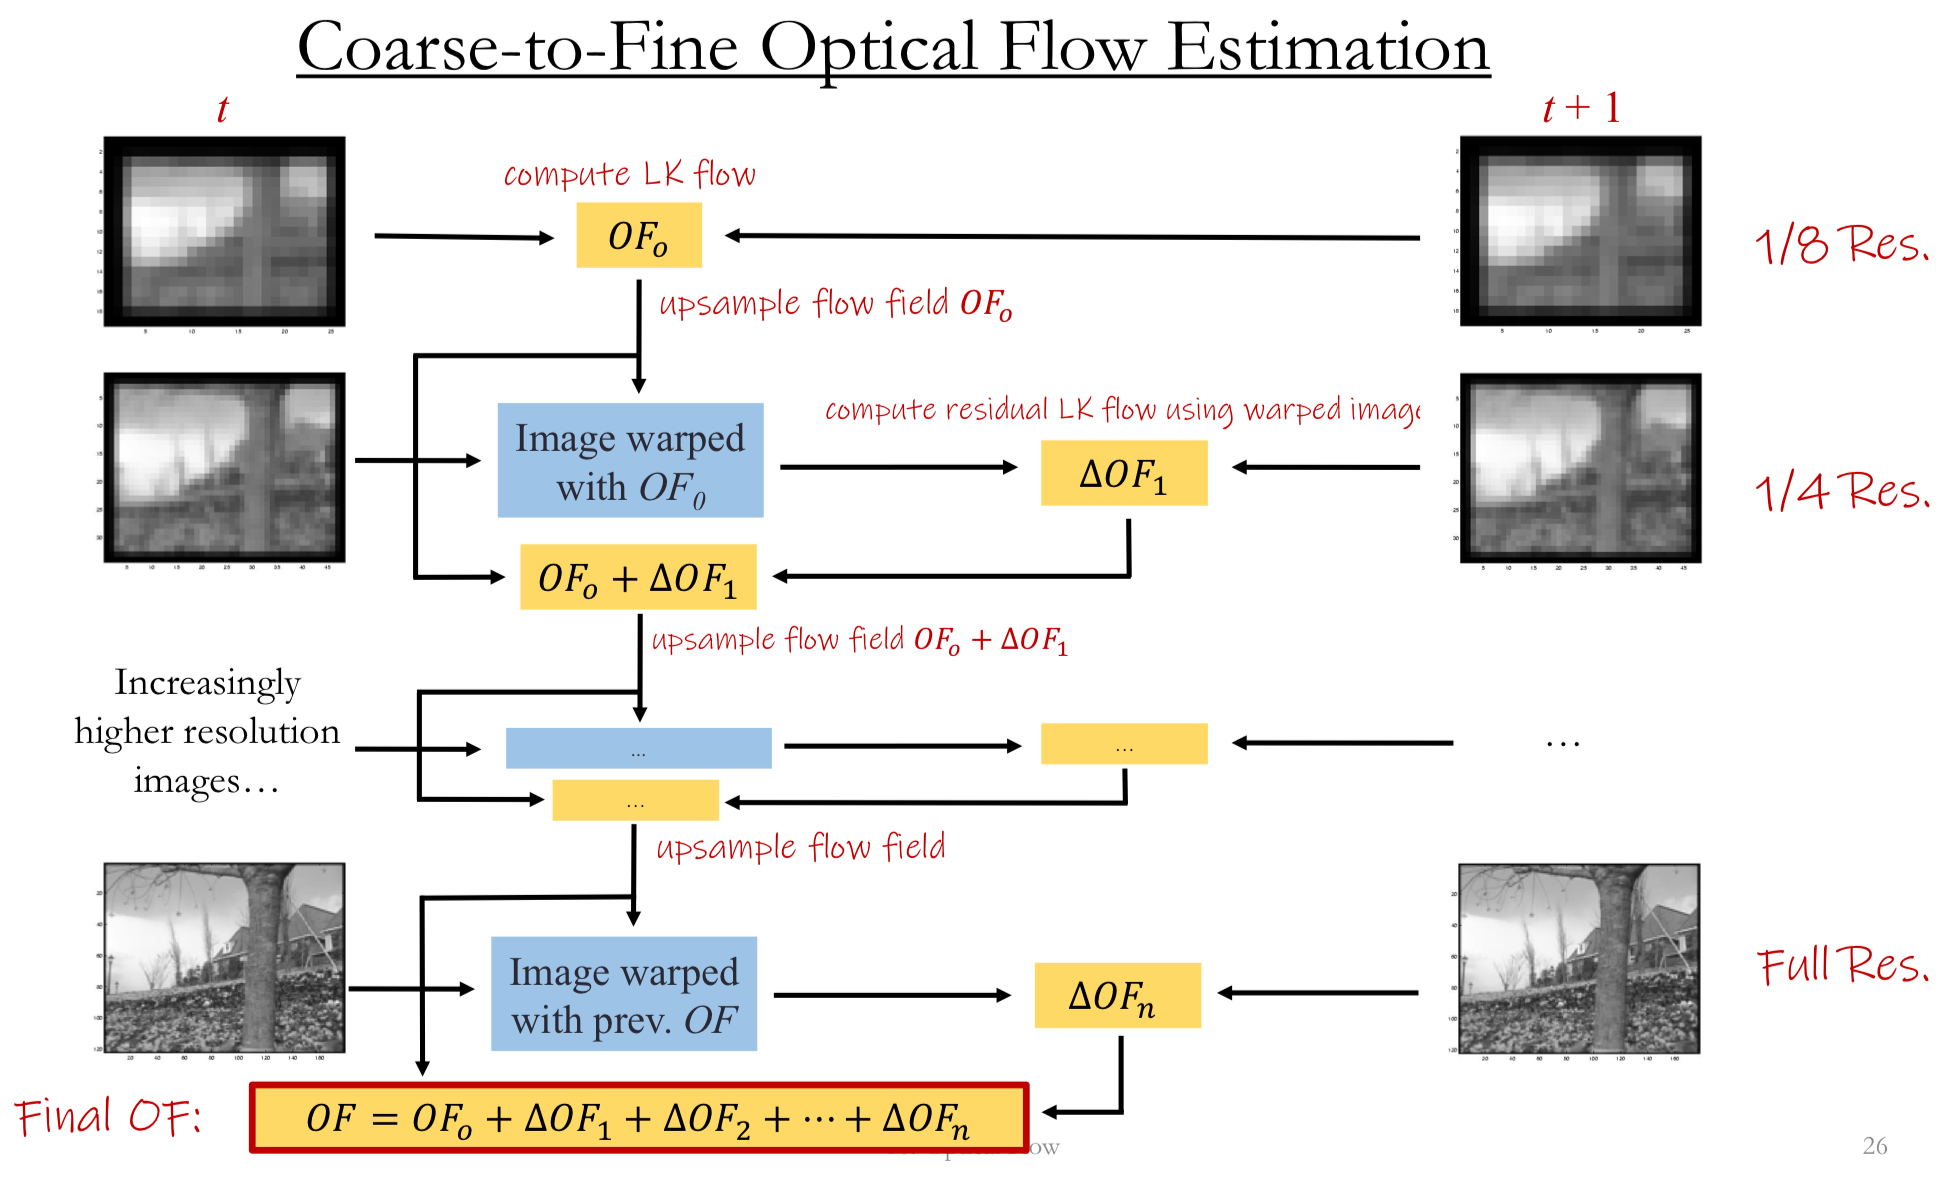
\includegraphics[scale=0.09]{coarse-to-fine-flow-estimation.jpg} 
    \end{itemize}
    \item \keyword{Horn-Schunck}{Assumes smooth flow field}
    \begin{itemize}
        \item Minimization problem: Use gradient descent
        \[
            \min_{u,v} \sum_{i,j} (E_s(i,j) + \lambda E_d(i,j))
        \]
        \item $E_s(i,j) = \frac{1}{4} ((u_{ij} - u_{i+1,j})^2 + (u_{ij} - u_{i,j+1})^2 + (v_{ij} - v_{i+1,j})^2 + (v_{ij} - v_{v,j+1})^2)$
        \item $E_d(i,j) = (I_x u_{ij} + I_y v_{ij} + I_t)^2$
    \end{itemize}
    \begin{enumerate}
        \item Compute $I_x$, $I_y$, $I_t$ and initialize flow $u=v=\mathbf{0}$
        \item Do until converge: $\hat{u}_{kl} = \bar{u}_{kl} - k I_x; \hat{v}_{kl} = \bar{v}_{kl} - k I_y$
        \[
            k = \frac{I_x \bar{u}_{kl} + I_y \bar{v}_{kl}+I_t}{\lambda^{-1} + I_x^2 + I_y^2} \text{ where } \bar{u}_{kl} \text{ is local avg.}
        \]
    \end{enumerate}
    \begin{itemize}
        \item Choice of $\lambda$: When small, maximize smoothness
        \item Produces \textbf{dense flow}: Flow for all pixels
        \item Good for when image motion is small
    \end{itemize}
    \item Evaluation: Euclidean distance, Cosine similarity
\end{itemize}

\section{11. Tracking}
\section{12. Deep Learning}

\end{multicols*}
\end{document}
